\chapter{Binary sequence representation}
\label{kap:kap2}

This chapter is dedicated to the previous work on the implementation of the bit vector, data
structure that stores binary sequence supporting methods access, rank and select. As we have
shown in section~\ref{section:WaweletTree}, Wavelet tree can be used to build a vector
for the general alphabet from the bit vector implementation. This is, why it is of utmost
importance to dedicate time to efficient and fast bit vector implementation. In this
chapter, we shall describe the currently available implementations. Let us start with
the simple representation of bit vector, in which we simply store bits one after another.
Then we shall look at the succinct representation.

\section{Bit vector implementation}

\subsection{Rank}
\label{section:rank}

Regarding rank, we are concerned in fact in two different methods namely $rank_0(i)$ and
$rank_1(i)$. It is easy to observe that following equation holds:

                    $$rank_1(i) = i - rank_0(i)$$

so it is enough to provide only the implementation of $rank_1(i)$.
There are two straightforward solutions we can begin with to support rank on bit vector
$B$. The first is to store no additional information. Every time we are asked
for $rank_c(i)$, we run through all bits preceding $i$-th. This solution is not very
practical for longer bit vectors but it does not add any additional space. The second
approach is to precompute rank up to every bit. This enables us to answer rank in constant
time as it consists of only one constant lookup. However, the space needed to support this
solution is $(|B|\cdot\log |B|)$. These two solutions can be combined together to obtain an
idea of the practically sound solution. We will store the precomputed rank, but not for every
bit. Instead, we choose a constant $k$ and precompute rank only for every $k$-th bit. This
enables answering rank in time $\mathcal{O}(k)$ and uses $\mathcal{O}((n/k)\log(n))$ of memory.

\subsection{Select}
\label{section:select}

It is important that the select method is working much like an inverse to rank. This is given
by the fact that

                $$rank_c(select_c(i)) = i$$.

Thanks to rank being a nondecreasing function, it is possible to binary search for the result
of $select_c(i)$. This can be nicely combined with the solution from the previous
section~\ref{section:rank}. At first, we binary search for the solution in the samples of rank
on the beginnings of every $k$-th bit. When we identify the correct block of $k$ bits, where
the answer is located, we simply linearly scan for the solution. This solution is not asking
for any additional memory on top of the space used for rank. The answer can be given in time
$\mathcal{O}(\log(n/k)+k)$.

\section{Succinct representation}

The main idea of \textit{RRR} is to split the bit sequence into blocks of constant length $b$.
This length is a parameter of the algorithm and can be chosen. After this, instead
of storing a single block as a bit sequence, we store each block encoded as a pair
of numbers $(c, o)$. Here, $c$ labels the class of the block and $o$ an offset into
the sequence of all blocks in this particular class. Most of the time, the $c$ is equal
to the number of ones in the block. Offset, on the other hand, is the index of block in
the sequence of all the blocks with $c$ ones, lexicographically sorted. Note that
class $c$ has a size

                $${b\choose c}$$.

The offset is then be bounded by:

				$$0 \leq o < {b\choose c}$$.

The process of obtaining $c$ and $o$ from the raw representation of block is called
\textit{encoding}. The opposite process is called \textit{decoding}. Although we would
like both processes to be fast. We do the encoding just once, at the initial construction
of the bit vector. On the other hand, decoding is done any time we are accessing particular
bit in $B$ so it is more important for us to optimise so that decoding is as fast as possible.

For smaller block sizes, such as $b\leq 15$, it is in most cases reasonable to
generate two helper tables. One is named $T_e$ used for the encoding, where we can
index using the block casted to a number and get this particular block's offset.
The class can be computed trivially by counting a number of ones. The other table
named $T_d$ is two dimensional. In position $T_d[c][o]$ we store the block that
is associated with $(c, o)$. In other words, this is a block containing $c$ ones
and at the same time being $o$-th in the sequence of all lexicographically sorted
blocks containing $c$ ones. Both these tables $T_e$ and $T_d$ can be computed
by generating all the possible blocks in lexicographical order before we even
obtain the sequence that we will want to represent. After this precomputation,
the encoding and decoding of a block takes constant time.

For small values of $b$ it is possible to store the whole table $T$ that helps us
encode and decode the block. For bigger $b$ it is not practical and many times
impossible to store a huge helper table. On the other hand, the bigger block size
yields a better compression because of the smaller per block overhead. This was
something that \cite{navarro2012fast} tried to achieve and came up with the method
we shall call \textit{on the fly-decoding}. This works by encoding and decoding without
the need for the helper table. Instead, it relies on a bit by bit decoding of the block
thus taking $\mathcal{O}(b)$ time instead of constant time with the use of table.

Idea is that we decode the block from the beginning, bit by bit until the end. On every bit,
we consider putting a zero bit on this position and count $comb$ -- the number of all
combinations how the block can look in this scenario. If the sequence number of the block --
$o$ is bigger than this number, we know that the decoded block will have one bit on this place.
We proceed by subtracting the number $comb$ from $o$ and proceed sequentially further.

After slicing the sequence $B$ to blocks, we need to find a way how to store pairs $(c, o)$.
We shall store all the classes and offsets in separate arrays $C$ and $O$. The array $C$ shall
be implemented as an array of fixed length elements with a length equal to
$\lceil \log_2(b)\rceil$. The array $O$ shall be on the other hand implemented as an array of
variable length elements with the size needed to store $i$-th element $O[i]$ being
$\lceil \log_2{b\choose C[i]}\rceil$.

To provide access to concrete bit, we need at first find out at which block this bit is located.
Let this be $i$-th block. To decode the block we at first need to get corresponding $C[i]$ and
$O[i]$ and then we can use a precomputed table $T_d$ that matches $(c_i, o_i)$ to the original
block. Obtaining $C[i]$ is trivial as it is at a fixed offset in memory. Getting the value of
$O[i]$ is harder as it is not at a known offset but generally on an offset that can be computed
as

                $$\sum_{j=1}^{i-1} \lceil\log_2{b\choose C[i]}\rceil$$

but is not known previously. To compute it without any precomputed information,
we need to basically one by one skip over elements that come before $O[i]$.
Note that to compute the previous sum, we need only successive information from $C$ so these
accesses are quite cache-friendly and fast. However, to access the $i$-th block, we need in the
worst case to look at all the elements of $C$ and this takes $\mathcal{O}(n/b)$ time. To support
this version of access, we need to store the arrays $C, O$ and helper table $T_d$. We shall
now argue about the size of these structures. The size of these structures is
as follows:

$C$ is array of $\lceil n/b \rceil$ elements of fixed size $\lceil \log(b+1) \rceil$.

For array $O$ we argue that its size is bounded by

% TODO: pridat vysvetlenie
\begin{align*}
    \sum_{i=1}^{n/b} \bigg\lceil{\log b\choose c_i}\bigg\rceil
    &\leq \sum_{i=1}^{\lceil n/b \rceil} \log {b\choose c_i} + \lceil n/b \rceil \\
    &= \log\prod_{i=1}^{\lceil n/b \rceil} {b\choose c_i} + \lceil n/b \rceil \\
    &\leq \log{n\choose \#_1(B)} + \lceil n/b \rceil &\leq nH_0(B) + \lceil n/b \rceil
\end{align*}

where $\#_1(B)$ denotes the total number of ones in $B$. We obtained (someref) using the
observation that ${b\choose c_i} {b\choose c_j} \leq {2b\choose c_i+c_j}$. This can be seen
when we interpet the left side of the equation as number of ways we can choose $c_i$ elements
from $b$ elements and $c_j$ elements from another $b$ elements. This is all contained in the
right side of equation that definitely includes all these combinations.

$T_d$ is storing $2^b$ entries and each entry is using $b$ bits of storage.
The total space used is then $nH_0(B) +  \lceil n/b \rceil + \lceil \log(b+1) \rceil + b2^b$.

To speed up the process of accessing block, we will help ourselves
store the pointers into every
$k$-th element of $O$. Effectively dividing the process of locating $O[i]$ into two
parts. The first is to find the nearest pointer leading to element before $i$ and
then move at most $k$ places. This additional structure of roughly $\frac{n}{bk}$ integers
takes the space $\mathcal{O}(\log(n)\cdot \frac{n}{bk})$.

\begin{figure}
	\centerline{
		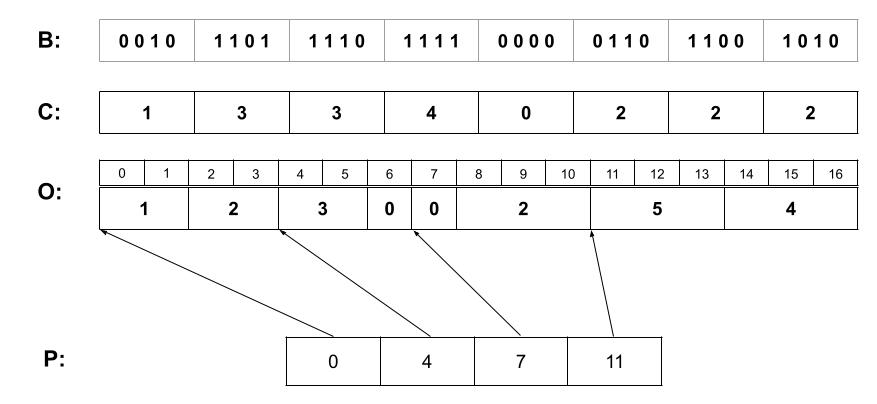
\includegraphics[width=0.9\textwidth, height=0.3\textheight]{images/rrr}
	}
	\caption[TODO]{RRR implementation. $B$ shows the original bit sequence cut to
    blocks. $C$ stores the class which is in this case number of ones in the block.
    $O$ uses variable number of bits per entry, in general $i$-th entry uses
    $\lceil \log_2{b\choose C[i]}\rceil$ bits. For $k=2$ we can see a helper array $P$
    storing bit offsets into every $k$-th element namely $0, 2, 4\ldots$
	}
	\label{obr:RRRFinal}
	% source at https://docs.google.com/drawings/d/1f1M7e-dZIiIZh1RdgqnmptF3xWZBKqjms3f_aQwVMhg/edit
\end{figure}

\section{Practical considerations}

\subsection{Block size}

First and one of the most important parameters of RRR implementation is the block
size $b$ used. The on the fly decoding has some advantages and disadvantages. The
biggest advantage is that it allows us to use a bigger block size $b$. The disadvantage
is that it takes $\mathcal{O}(b)$ steps to decode the block. Furthermore, the decoding
contains branching and it is hard to parallelize the steps in some meaningful way.
Note that decoding is faster if we want to access the element close to the beginning of
the block as we can stop the process when we obtain this bit.

%%% OTHER STUFF

divide the bit vector into nonoverlaping parts consisting of $k$
successive bits and name this \textit{superblock}. If the number of bits in the bit vector
is not divisible by $k$ we simply left the last superblock shorter. We now compute the rank
value only for the beginnings of superblocks.